\section{Introduction}
We compile trait data for terrestrial vertebrates. We impute missing values and test the robustness of imputatutions.


\section{Methods}

\subsection{Ecological trait data collection}

\subsubsection{Trait choice}
I collated ecological trait data for terrestrial vertebrates from published databases and unpublished sources (Table \ref{datasources}). Targeted traits related to species life history (body mass, longevity, litter or clutch size, trophic level, diet) and to their habitat preferences (habitat breadth, habitat specialisation). Traits were selected for three main reasons: (1) estimates were available for many species; (2) estimates were available across all four terrestrial vertebrate classes, allowing cross-classes comparative analyses (true for all traits except diet); (3) selected traits have been shown to be response or effect traits in other studies or are related to response or effect traits (Table in Chapter 1). 

% Elaborate on relevance of these traits.

% Table of sources.
\begin{table}[h!]
\renewcommand{\baselinestretch}{1}
\renewcommand{\arraystretch}{1.5}
\begin{center}\fontsize{9}{11}\selectfont
\caption[Data sources for trait compilation]{\textbf{Data sources for trait compilation.} BM: body mass; BL: body length; L: longevity or maximum longevity; GL: generation length; LCS: litter or clutch size; TL: trophic level; Di: diet; DA: diel activity; RS: range size; H: habitat data. In bold, the traits of interest. Other traits were added for potential correlations in further imputations.} 
\label{datasources}
\begin{tabular}{|l|c|c|c|c|c|c|c|c|c|c|c|c|}
\hline
\multicolumn{1}{|c|}{\multirow{2}{*}{\textbf{Sources}}} & \multirow{2}{*}{\textbf{Taxa}} & \multicolumn{9}{c|}{\textbf{Traits}} & \multirow{2}{*}{\textbf{RS}} & \multirow{2}{*}{\textbf{H}} \\ \cline{3-11}
\multicolumn{1}{|c|}{} &  & \textbf{BM} & BL & \textbf{L} & MA & GL & \textbf{LCS} & \textbf{TL} & \textbf{Di} & \textbf{DA} &  &  \\ \hline
Amphibio & \multirow{4}{*}{Amphibians} & \checkmark & \checkmark & \checkmark & \checkmark &  & \checkmark &  & \checkmark & \checkmark &  &  \\ \cline{1-1} \cline{3-13} 
Cooper &  &  & \checkmark &  &  &  & \checkmark &  &  &  & \checkmark &  \\ \cline{1-1} \cline{3-13} 
Senior &  &  & \checkmark &  &  &  &  &  &  &  &  &  \\ \cline{1-1} \cline{3-13} 
Bickford &  &  & \checkmark &  &  &  &  &  &  &  & \checkmark &  \\ \hline
Elton & \multirow{2}{*}{Birds} & \checkmark &  &  &  &  &  &  & \checkmark & \checkmark &  &  \\ \cline{1-1} \cline{3-13} 
Butchart &  & \checkmark &  & \checkmark &  &  &  &  &  &  &  &  \\ \hline
Pantheria & \multirow{5}{*}{Mammals} & \checkmark & \checkmark & \checkmark & \checkmark &  & \checkmark & \checkmark &  & \checkmark &  &  \\ \cline{1-1} \cline{3-13} 
Kissling1 &  &  &  &  &  &  &  & \checkmark & \checkmark &  &  &  \\ \cline{1-1} \cline{3-13} 
Kissling2 &  &  &  &  &  &  &  & \checkmark & \checkmark &  &  &  \\ \cline{1-1} \cline{3-13} 
Elton &  & \checkmark &  &  &  &  &  &  & \checkmark & \checkmark &  &  \\ \cline{1-1} \cline{3-13} 
Pacifici &  & \checkmark &  & \checkmark & \checkmark & \checkmark &  &  &  &  &  &  \\ \hline
Scharf & \multirow{8}{*}{Reptiles} & \checkmark &  & \checkmark & \checkmark &  & \checkmark & \checkmark &  & \checkmark &  &  \\ \cline{1-1} \cline{3-13} 
Meiri &  &  &  &  &  &  &  & \checkmark &  & \checkmark &  &  \\ \cline{1-1} \cline{3-13} 
Vidan &  &  &  &  &  &  &  &  &  & \checkmark &  &  \\ \cline{1-1} \cline{3-13} 
Stark &  & \checkmark &  & \checkmark &  &  & \checkmark &  &  & \checkmark &  &  \\ \cline{1-1} \cline{3-13} 
Schwarz &  &  &  &  &  &  & \checkmark &  &  &  &  &  \\ \cline{1-1} \cline{3-13} 
Novosolov1 &  & \checkmark &  &  &  &  &  & \checkmark &  &  & \checkmark &  \\ \cline{1-1} \cline{3-13} 
Novosolov2 &  &  &  &  &  &  & \checkmark &  &  &  &  &  \\ \cline{1-1} \cline{3-13} 
Slavenko &  & \checkmark &  &  &  &  &  &  &  &  &  &  \\ \hline
Myhrvold & Amniotes & \checkmark & \checkmark & \checkmark & \checkmark &  & \checkmark &  &  &  &  &  \\ \hline
IUCN & Vertebrates &  &  &  &  &  &  &  &  &  & \checkmark & \checkmark \\ \hline
\end{tabular}
\end{center}
\end{table}

\subsubsection{Compilation methods}

\paragraph{Continuous traits.}
All continuous traits (body mass, litter or clutch size, longevity) were averaged within species when different sources provided estimates. Longevity and maximum longevity were assumed to provide the same information and were also averaged within species.
% Here what did I do when body mass or longevity was given by sex?
In addition, I compiled traits that were potentially correlated to either body mass or longevity, to be used as potential predictors in imputations of missing values. As such, body length information was compiled when available, as well as generation length or age at sexual maturity. Finally, species geographical range sizes were calculated from distribution data, extracted from the IUCN Red List.

\paragraph{Categorical traits.}
Diet was available for all classes except reptiles. Species diet was described as a binary variable recording whether food items were known to be consumed by a species or not. % Food items?
For amphibians and birds, trophic levels were partly inferred from the diet. 
Species habitat preferences were compiled from IUCN habitat data files and were described as a binary variable recording whether a species was known to occur in a particular habitat. 

I used these compiled traits to design three other ecological variables. Diet breadth was calculated as the number of food items a species was recorded to ingest. Similarly, habitat breadth was calculated as the number of habitats a species was known to use. Weights were assigned to each habitat in this calculation depending on whether the habitat was recorded to be suitable or marginal for each species; outcomes were not sensitive to different weight choices (see SI). Finally, a broad degree of habitat specialisation was produced. If any artificial habitat was recorded to be suitable, species were reported to be generalists; else, they were natural habitat specialists.

More details on how diet and habitat variables were compiled are provided in the SI.
%Due to the lack of comprehensive diet information readily available for reptiles, and despite compilation efforts for other classes, diet was excluded from further analyses in all four classes.

\subsection{Phylogenies}
I obtained phylogenetic trees for birds, amphibians, mammals and squamates from Hedges et al (2015)
(available at http://www.biodiversitycenter.org/ttol, downloaded 06/07/2018).

\subsection{Taxonomic synonymy}

\subsubsection{Extracting synonyms and harmonising taxonomy in trait datasets.}

\paragraph{Procedure}
Across the different sources, similar species could appear under different binomial names. Taxonomic synonymy created `pseudoreplicates' of the same species, overall falsely increasing the total number of species and artificially inflating the amount of missing trait values. As such, taxonomic synonymy was a major issue; due to the large number of species across datasets, extensive manual checks could not be applied. The presence of typos in species names had the same effect as synonymy. I attempted to correct for taxonomy by developping an automated procedure, complemented with a few manual entries. Obvious cases where vernacular names had been entered in the place of binomial names were also treated manually; when possible, I best assigned binomial names to species common names. 

The automated procedure consisted in extracting species accepted and synonymic binomial names from the IUCN Red List or from the Integrated Taxonomic Information System database (ITIS), using the rredlist and taxize R packages. For each class, I started by generating a list of all binomial names figuring across datasets. These `original' binomial names were corrected for typos using gnr\textunderscore resolve (taxize R package). For each of these corrected names, the IUCN RedList was queried and synonyms and accepted names were stored. When species were not found in the IUCN Red List, information was extracted from ITIS. When species were not found in ITIS either, corrected names were assumed to be accepted. Family and order information was extracted using the same procedure and some entries were completed using the Global Biodiversity Information Facility taxonomic backbone (https://www.gbif.org/tools/species-lookup). Taxonomy across datasets was finally homogenised by replacing recorded synonyms with their accepted scientific names. Overall, this procedure reduced the total number of species figuring in trait datasets (Table XXX).

Nevertheless, additional manual checks were required to make sure that all vertebrate species appearing in PREDICTS were represented in the trait datasets. Taxonomic synonymy was resolved manually for PREDICTS species that did not match any species in the trait datasets. Information was extracted from other diverse sources (such as The Reptile Database; Avibase; AmphibiaWeb). The need to apply additional manual inputs underlined the fact that the automated procedure to correct for taxonomic synonymy was not optimal. The Red List and ITIS were not comprehensive taxonomic sources for accepted names and synonyms. Species `pseudoreplication' is likely to have persisted to a degree. 

% Result table: delta number of species 
% Extract of synonym dataset

\paragraph{Increase in trait coverage due to taxonomic correction}
Across all classes, correcting for taxonomy overall increased trait coverage, measured as the percentage of species for which information was not missing. For mammals and birds, intial trait coverage was high. On the other hand, the variability in coverage was much higher for reptiles and amphibians.

\begin{figure}[h!]
\centering
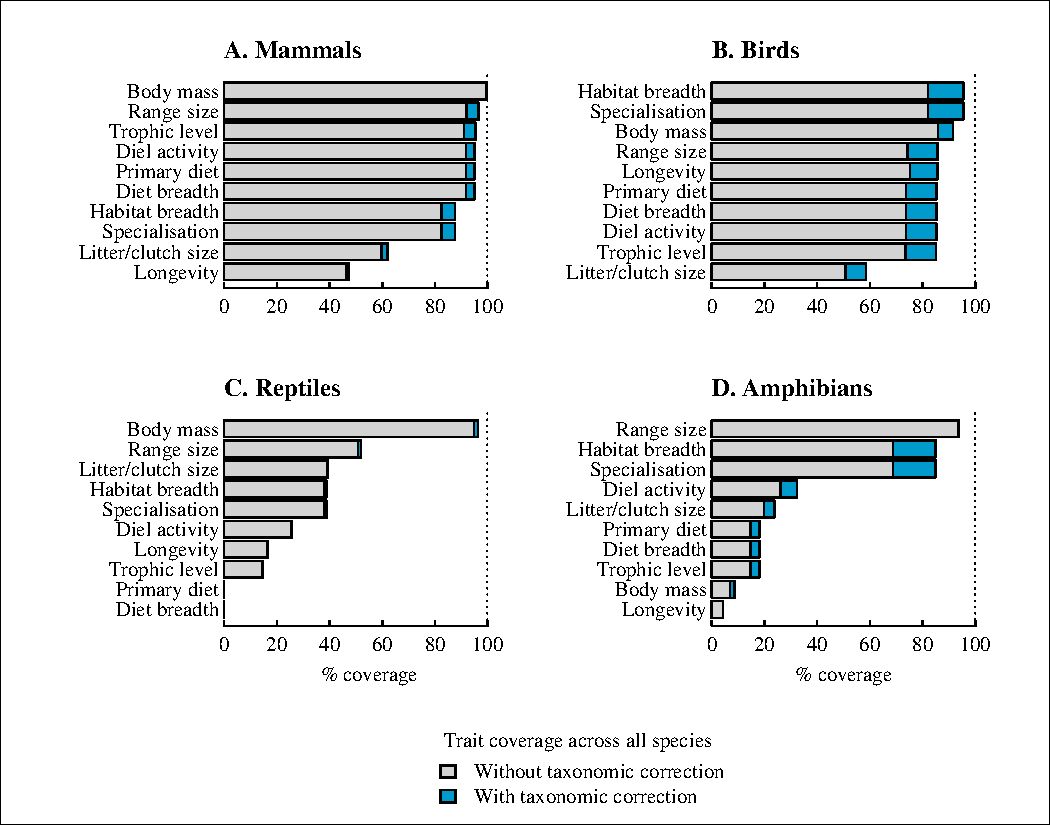
\includegraphics[scale=0.85]{figures/chapter2/Target_traits_All_species_coverage}
\caption[Trait coverage across all species before and after taxonomic correction]{\textbf{Trait coverage across all species before and after taxonomic correction.} Trait coverage is defined here as the percentage of species for which trait information is available. Correcting for taxonomic synonymy improved trait coverage in most cases.}
\end{figure}

For species figuring in PREDICTS, trait coverage disproportionally increased for reptiles and amphibians.

\begin{figure}[h!]
\centering
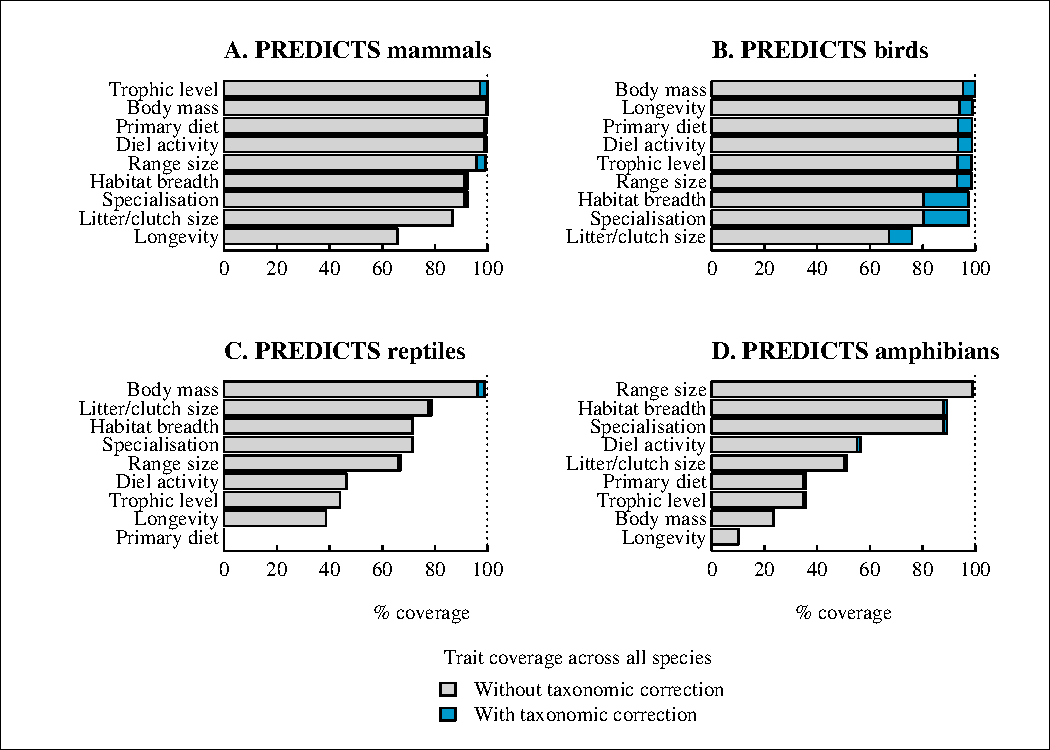
\includegraphics[scale=0.85]{figures/chapter2/Target_traits_Predicts_species_coverage}
\caption[Trait coverage across PREDICTS species before and after taxonomic correction]{\textbf{Trait coverage across all species before and after taxonomic correction.} Trait coverage is defined here as the percentage of species for which trait information is available. Correcting for taxonomic synonymy improved trait coverage in most cases.}
\end{figure}



\subsubsection{Harmonising taxonomy in phylogenetic trees and increasing species representation.}

\paragraph{Taxonomic correction across tip labels.} 
To correct for taxonomy across phylogenies, I applied the same method as above, replacing synonyms by their identified accepted names in trees' tip labels. In some cases, this procedure assigned the same accepted name to different phylogenetic tips. This was the case for 2.6\% of mammalian, 1.5\% of avian, 1\% of amphibian and  1.5\% of reptilian species, which then had multiple phylogenetic positions. In other words, replicated tips appeared. Most of these replicated species had two different positions (see table). For each replicated tip, I selected one tip to conserve and dropped other tips from the phylogenies (Figure \ref{chart_phylorep}). If replicated tips were sister clades, the tip to conserve was chosen randomly among the replicates. Else, I chose to conserve the tree tip whose position was closest to the position of the same tip in the uncorrected tree, when present. In all other few cases, tips to drop were chosen randomly. Further details on how replicated tips were dropped are available in the SI.
\vspace{0.5cm}
\begin{figure}[h!]
\centering
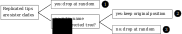
\includegraphics[scale=0.7]{figures/chapter2/chart_phylorep}
\caption[Procedure followed to drop replicated tips from phylogenies]{\textbf{Procedure followed to drop replicated tips from phylogenies.} Most of these were replicated twice, and were sister clades. In that case, tips to drop were chosen randomly, as it did not affect the `true' phylogenetic position of the species (1). When replicated were not sister clades, I kept the tip whose position was closest to the position of the same tip in the uncorrected tree (2). In a few cases, the corrected name did not appear in the original tree. Those were problematic cases, and the tips to drop were chosen randomly (3). Nevertheless, occurences of that third case were rare (see table). See SI for more case examples and more details on the procedure.}
\label{chart_phylorep}
\end{figure}

% Table with number of replicates, number of which were sister clades:
% Number of repliated tips, number that are sister clades, number that are truly pbmatic
% occurences of number of replicates.

\paragraph{Random species attachments.} Some species in the trait datasets were not represented in the phylogenies. When applicable, and to increase representation, these species were attached to their genera in the trees at a random position (phytools). Only a small fraction of species that had no initial phylogenetic representation were randomly attached to their genera (Table \ref{random_attachments_phy}).
Overall, correcting for taxonomy improved species representation in the phylogenies (Figure \ref{species_rep_phylo}). For amphibian and reptilian PREDICTS species, representation disporprotionally increased (minimum representation: 73\%,for PREDICTS amphibians). 

\begin{table}[h!]
\renewcommand{\baselinestretch}{1}
\renewcommand{\arraystretch}{1.5}
\begin{center}\fontsize{9}{11}\selectfont
\caption[Species representation in phylogenetic trees (corrected taxonomy)]{\textbf{Species representation in phylogenetic trees (corrected taxonomy).} The number of species randomly attached to their genera anged from 17 (amphibians) to 611 (reptiles). Finally, most avian and mammalian species were placed in the phylogenies, whereas more than half reptilian and amphibian species were not.} 
\label{random_attachments_phy}
\begin{tabular}{|l|l|l|c|l}
\cline{1-4}
\multicolumn{1}{|c|}{\textbf{Class}} & \multicolumn{1}{c|}{\textbf{Initially not in tree}} & \multicolumn{1}{c|}{\textbf{Randomly attached}} & \textbf{No final representation in tree} &  \\ \cline{1-4}
Amphibians                  & 59\% (4062 of 6927)                           & 0.4\% (17 of 4062)                     & \textbf{58\%}             &  \\ \cline{1-4}
Birds                       & 18\% (2084 of 11637)                          & 4.8\% (100 of 2084)                    & \textbf{17\%}             &  \\ \cline{1-4}
Mammals                     & 7.4\% (407 of 5502)                           & 23\% (94 of 407)                       & \textbf{5.7\%}            &  \\ \cline{1-4}
Reptiles                    & 62\% (6391 of 10334)                          & 9.6\% (611 of 6391)                    & \textbf{56\%}             &  \\ \cline{1-4}
\end{tabular}
\end{center}
\end{table}

\begin{figure}[h!]
\centering
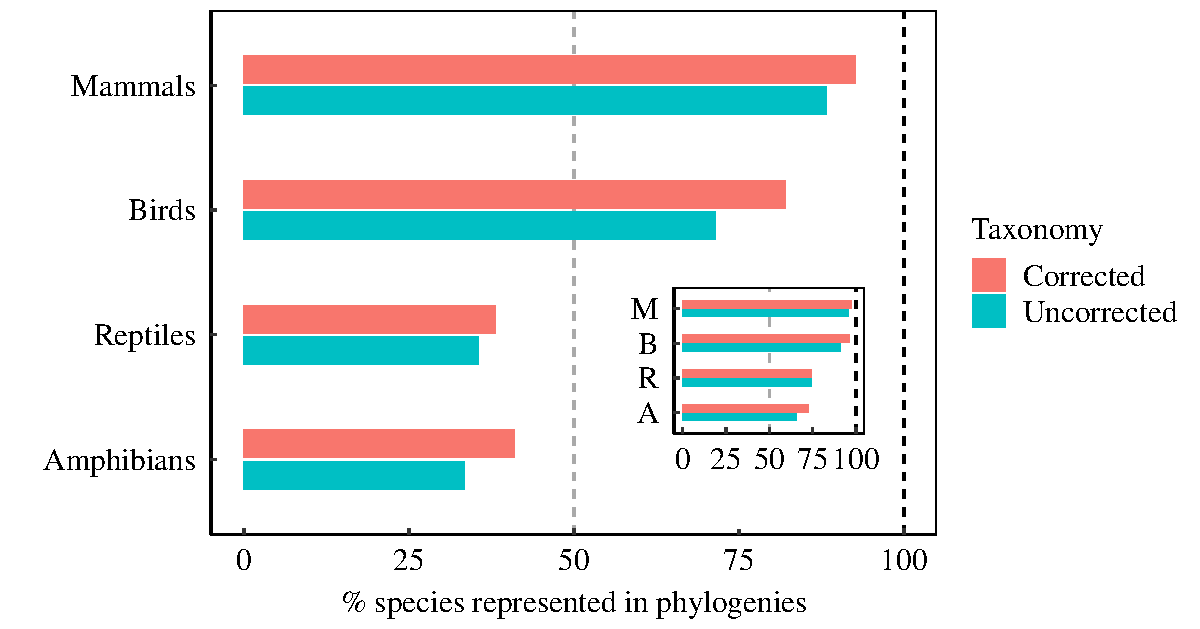
\includegraphics[scale=0.7]{figures/chapter2/Species_representation_phylo}
\caption[Percentage of species represented in the phylogenies for both corrected and uncorrected trait datasets]{\textbf{Percentage of species represented in the phylogenies for both corrected and uncorrected trait datasets.} Overall, taxonomic correction increased species representation in phylogenetic trees. Representation for mammals and birds was high (after taxonomic correction: 83\% of avian and 94\% of mammalian species had a phylogenetic position). On the other hand, reptiles and amphibians were poorly represented (after taxonomic correction: only 39\% of reptilian and 42\% of amphibian species were placed in phylogenetic trees). The inset barplot shows representation for species figuring in PREDICTS. For these, species presence in phylogenetic trees after correction was high across all classes, with a minimum representation of 73\% for amphibians.}
\label{species_rep_phylo}
\end{figure}


\subsection{Trait transformations}
Species for which all trait values were missing were filtered out. All continuous traits were log10 (except habitat, square root) and standardised to zero-mean and unit variance.

% Table with final number of species

\subsection{Imputation of missing trait values}

% TODO/
% finir coverage
% Randomness in missing trait values:
% 1) fill information across classes
% 2) randomness missing values <> taxonomy?
% 3)trait phylo signal
% 4) missForest imputations & imputation error / robustness. Compare with Rob's for mammals and birds.


\subsubsection{Randomness in missing trait values}

\subsubsection{Phylogenetic signal}

\subsubsection{Imputations of missing trait values}

I imputed missing values using random forest algorithms (missForest R package). For some traits, the phylogenetic signal (assessed using Pagel’s lambda) was strong, showing that they were highly evolutionary conserved. To account for phylogenetic relationships among species, phylogenetic eigenvectors were included in the random forest imputations as a supplementary predictor. Eigenvectors were extracted from the phylogenies using the PVR package (Santos, 2018). Penone et al showed that including 10 eigenvectors minimised the imputation errors – hence I included 10 eigenvectors. Plus best method with phylogenies.

Otherwise, traits for these sets of species were imputed without additional phylogenetic information, in a second round of imputations, with family, order, and genus as additional predictors.

Robustness of imputations

\section{Results}


\section{Discussion}
Discuss taxonomy and robustness of imputations

